% This is based on the LLNCS.DEM the demonstration file of
% the LaTeX macro package from Springer-Verlag
% for Lecture Notes in Computer Science,
% version 2.4 for LaTeX2e as of 16. April 2010
%%\author{Ivar Ekeland\inst{1} \and Roger Temam\inst{2}
%Jeffrey Dean \and David Grove \and Craig Chambers \and Kim~B.~Bruce \and
%Elsa Bertino}
%%
%\authorrunning{Ivar Ekeland et al.} % abbreviated author list (for running head)
%%
%%%%% list of authors for the TOC (use if author list has to be modified)
%\tocauthor{Ivar Ekeland, Roger Temam, Jeffrey Dean, David Grove,
%Craig Chambers, Kim B. Bruce, and Elisa Bertino}
%%
%\institute{Princeton University, Princeton NJ 08544, USA,\\
%\email{I.Ekeland@princeton.edu},\\ WWW home page:
%\texttt{http://users/\homedir iekeland/web/welcome.html}
%\and
%Universit\'{e} de Paris-Sud,
%Laboratoire d'Analyse Num\'{e}rique, B\^{a}timent 425,\\
%F-91405 Orsay Cedex, France}

% See http://www.springer.com/computer/lncs/lncs+authors?SGWID=0-40209-0-0-0
% for the full guidelines.
%
\documentclass{llncs}
\usepackage{hyperref}
\usepackage{amsmath}
\usepackage{graphicx}
\usepackage{caption}
\usepackage{amssymb}
\usepackage{subfig}
\usepackage{verbatim}
\usepackage{array}


%\usepackage{authblk}


\begin{document}

\title{Atomic Swaps}
\maketitle              % typeset the title of the contribution

\begin{abstract}
\end{abstract}

\section{Introduction}\label{sec:intro}
An atomic swap enables involving parties to exchange cryptocurrencies, tokens on or off-chain without the involvement of a third party. Atomicity guarantees that either both sides of the swap happen, or neither. The risk of one party losing their assets is minimized. The concept of atomic swaps, which provides safe and quick trades, is being discussed since 2013\cite{altcoin}. Atomic swaps can be on-chain or off-chain. Off-chain swaps are instant, private and they almost doesn't incur any fees. Both type of swaps utilize hashed-time-locked-contracts (HTLCs) to guarantee that a party can't take any funds before providing his fund.


\section{Related Work}
Decred realized \textbf{the first on-chain atomic swap} between Decred and Litecoin~\cite{decred}. The need to mine new blocks to show the change of ownership can make the Decred's system slower. \textbf{The first on-chain Ethereum-Bitcoin atomic swap} is realized by Altcoin.io(REF!!). Lightning Labs performed \textbf{the first off-chain atomic swap} over the lightning network. Lightning network enables the off-chain exchange of coins  by creating payment channels between the trading parties. After the transaction is completed, the chains are updated and the channels are closed. Lightning network enables fast and scalable transactions and the involving parties don't have to pay transaction fees for every transaction.

%Their next goal: atomically swap any token for any other token, regardless of the blockchain it resides on.
Ethereum’s Raiden Network is analogous to Bitcoin’s Lightning Network and it provides instant, low-fee and scalable exchanges~\cite{Raiden}. The atomic swap of ERC20 tokens are performed on Raiden network.%Problem in decentralised exchanges: sacrificing transaction speed for settlement on-chain.
Zhang et al. propose Republic Protocol, which is a decentralized open-source dark pool protocol that provides atomic swaps of cryptocurrencies across Bitcoin and Ethereum blockchains~\cite{zhang2017republic}.%Republic: a  facilitating atomic swaps between cryptocurrency pairs across the . Trades are on a hidden orderbook and the matching is done using secure multiparty computation. It is a secure, decentralized, scalable dark pool protocol capable of handling billions in trading volume daily.
Their proposed system enables the exchange of Ether, ERC20 and Bitcoin over a decentralized dark pool. %execution without exposing price and volume, no trusted intermediary to operate a dark pool (dark pool = private exchanges where financial assets and instruments are traded and matched by an engine running on a hidden order book)Republic Protocol removes the risk of asset theft, confiscation or possibility of interference from a malicious exchange operator. Components: Decentralized hidden order book, Decentralized order matching, Atomic swap infrastructure, REN token nodes have no incentive to ignore an order, especially since they do not know the identity of the trader, nor the details of the order
In an atomic cross-chain swap setting, involving parties perform exchange across different blockchains like exchanging Bitcoin for Ether. In ~\cite{herlihy2018atomic}, a cross-chain swap is modeled as a directed graph where vertices correspond to the parties in the protocol and the arcs represent the transfers between them.
%An atomic swap protocol can be thought of as a trust-free, Byzantine-hardened form of distributed commitment. An atomic cross-chain swap is a special case of a distributed atomic transaction, although not all atomic transactions can be expressed as cross-chain swaps. If swaps are recurrent, then it would be useful to conduct swaps off‚-chain as much as possible, similar to the way that Lightning and Raiden networks support off‚-chain transactions for bitcoin and ERC20 tokens.

%FAIR EXCHANGE?
Œ%The fair exchange problem ~\cite{franklin1998secure}, ~\cite{micali2003simple} is a precursor to the atomic cross-chain swap problem. Alice has a digital asset Bob wants, and vice-versa, and at the end of the protocol, either Alice and Bob have exchanged assets, or they both keep their assets. In the absence of blockchains, trusted, or semi-trusted third parties are required, but roles of those trusted parties can be minimized in clever ways.

\section{Our Implementation}

\begin{itemize}
  \item ETH to ERC20 token atomic swap is implemented.
  \item ERC20 to ERC20 token atomic swap is implemented.
  \item One contract can perform several swaps. Each swap is assigned a swapID.
  \item Each swap has three states: OPEN, CLOSED or EXPIRED.
\end{itemize}

\begin{figure}[h!]
\centering
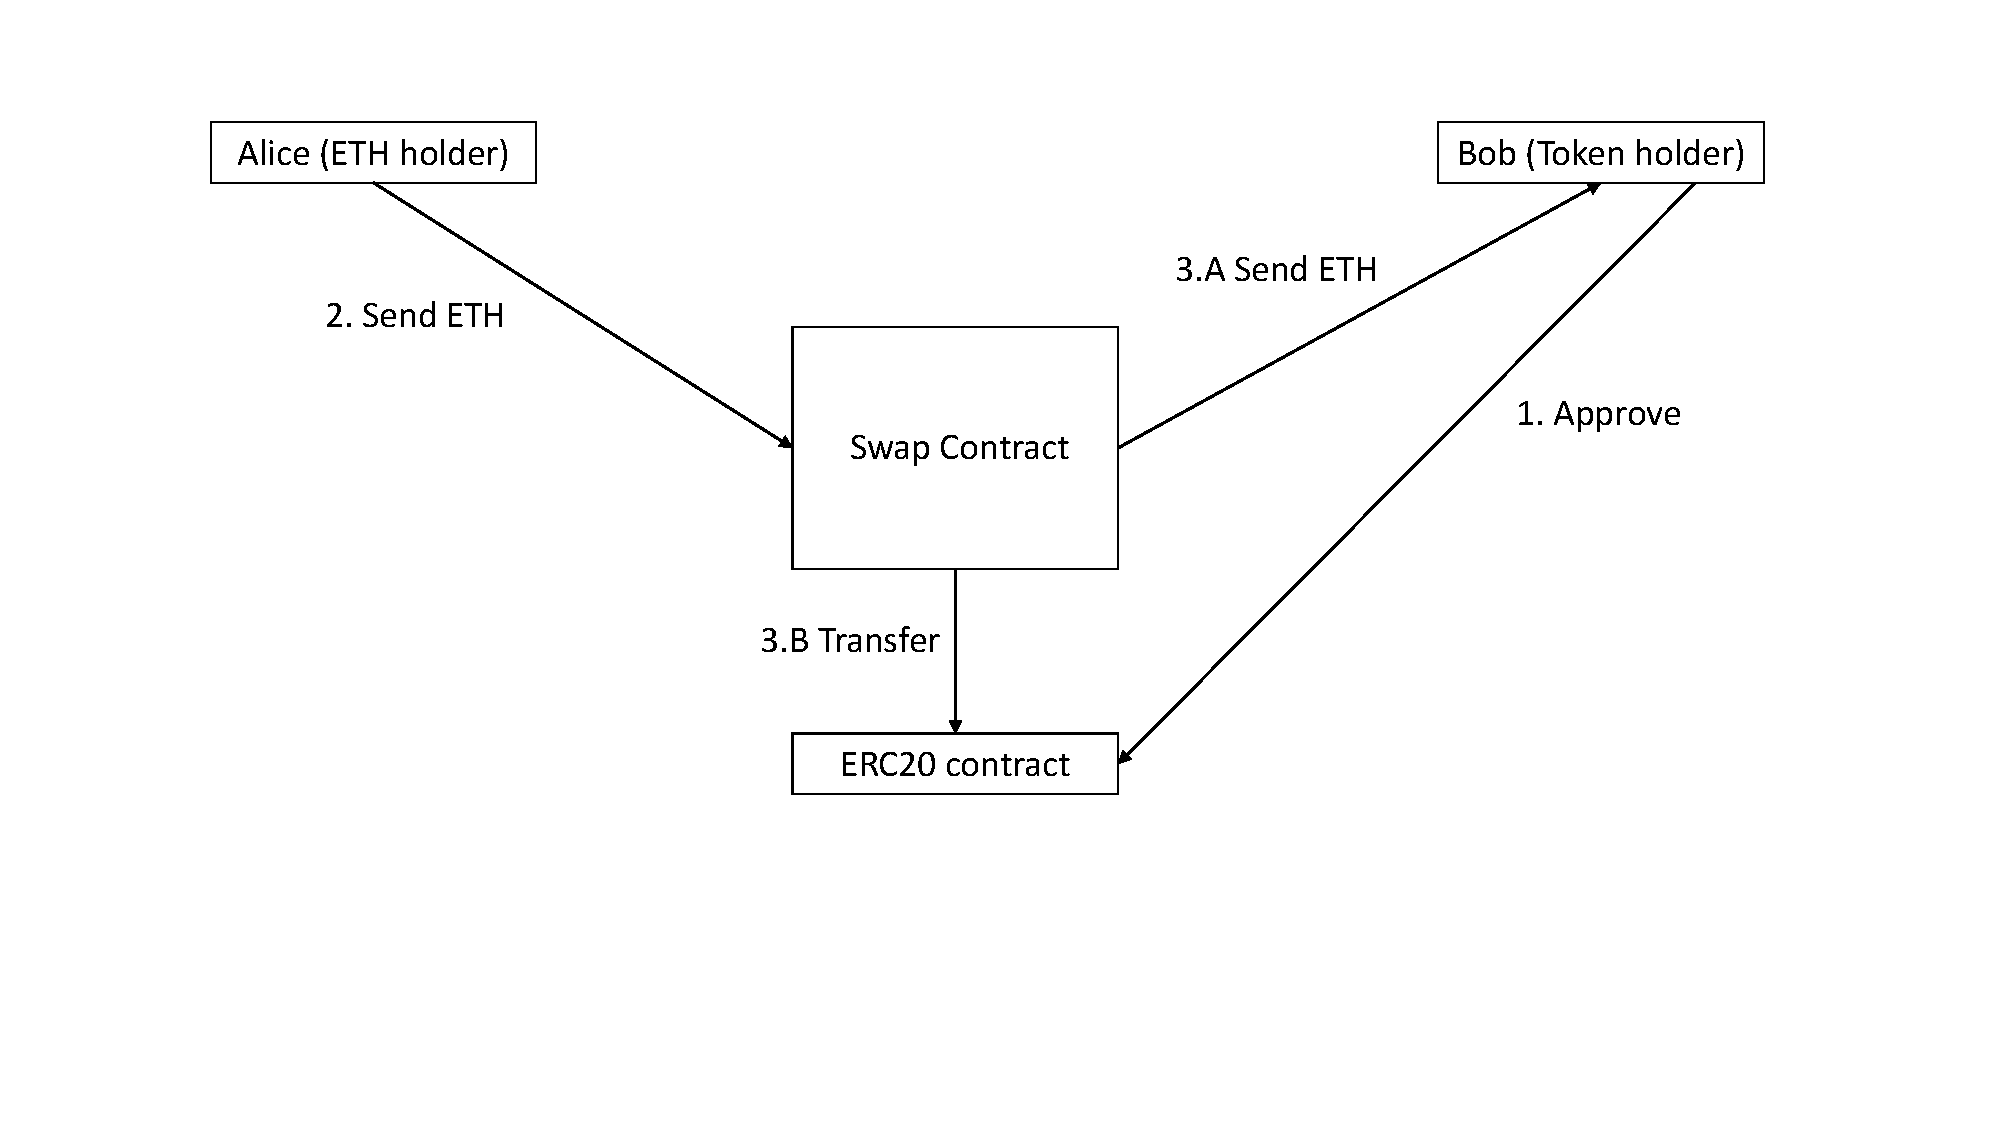
\includegraphics[width=1\textwidth]{approve}
\caption{approve}
\label{fig:withapprove}
\vspace{-10pt}
\end{figure}

\begin{figure}[h!]
\centering
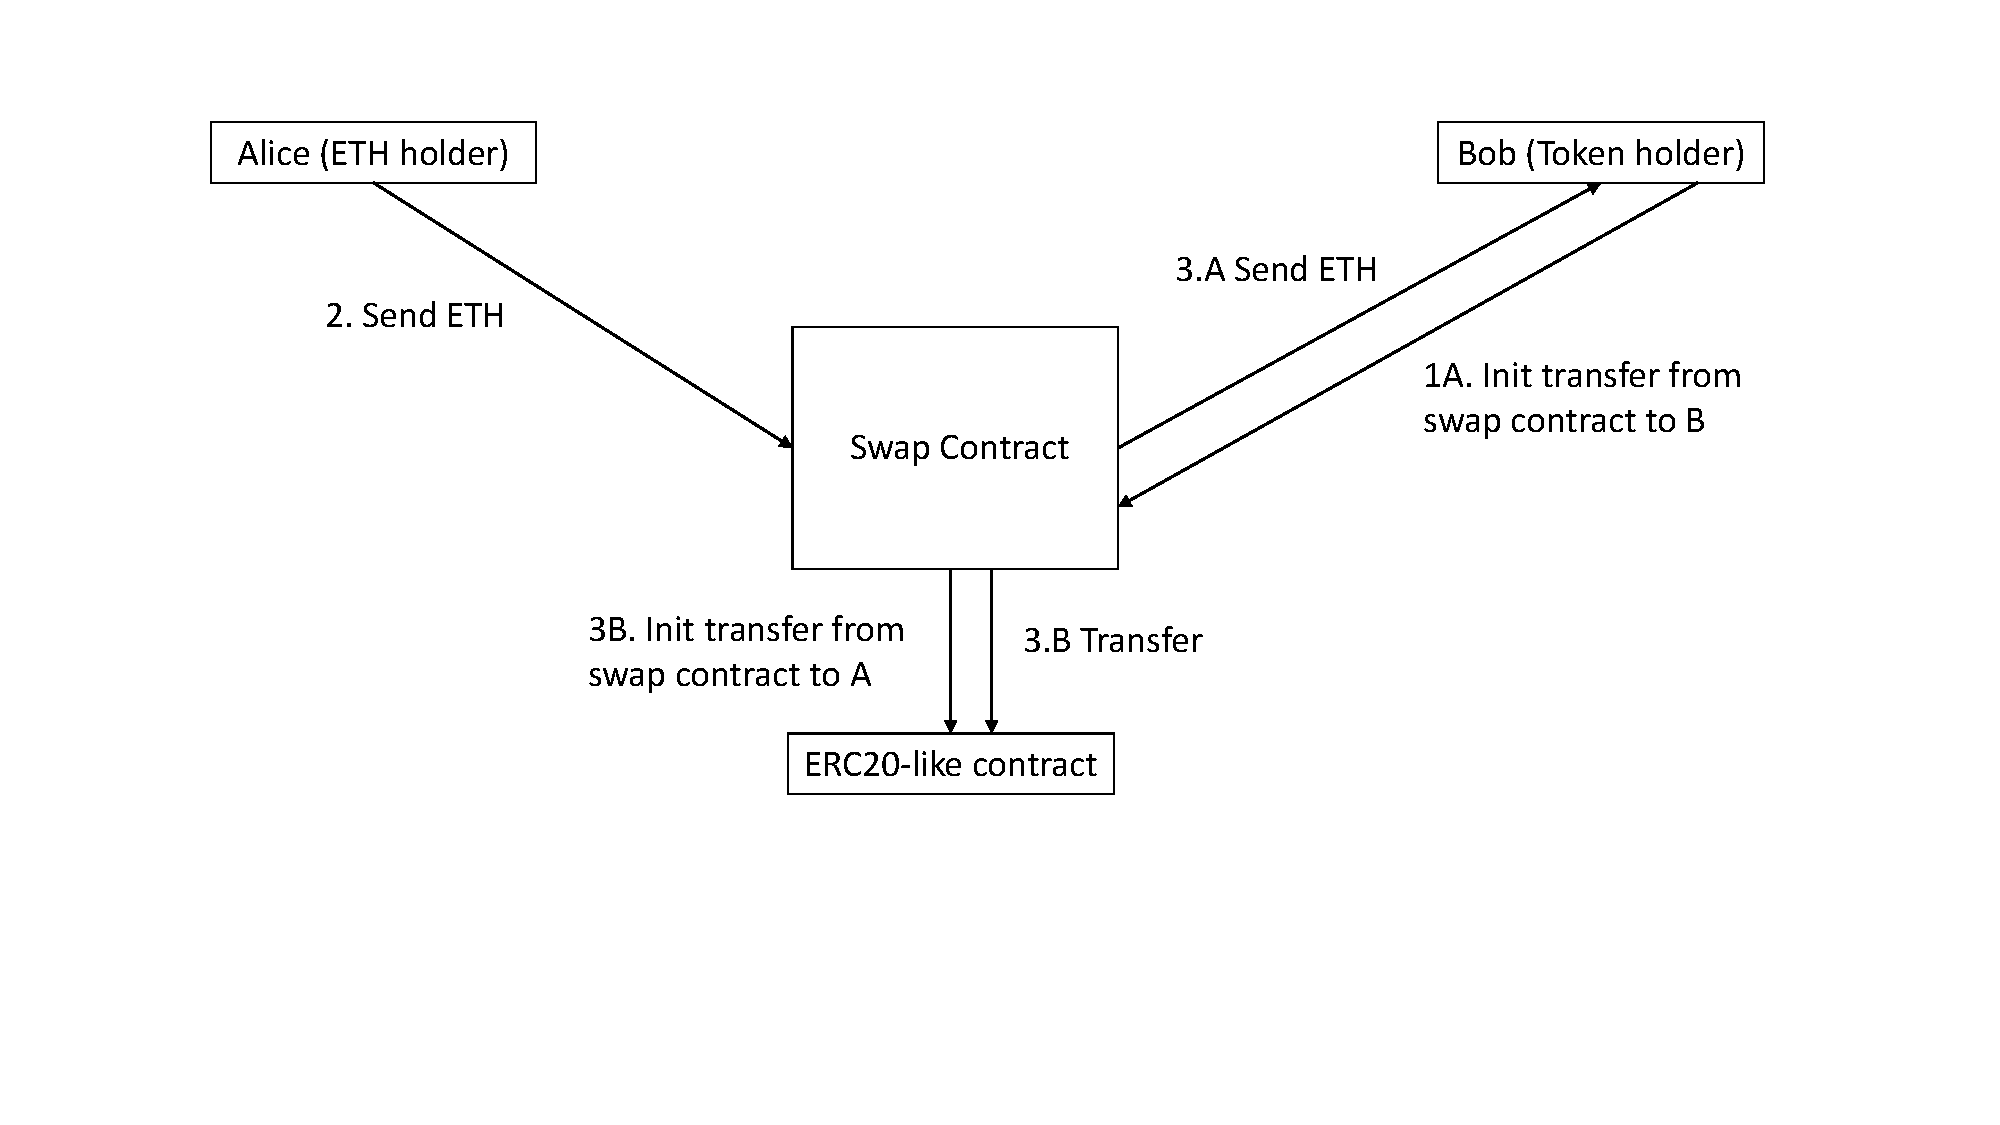
\includegraphics[width=1\textwidth]{withoutapprove}
\caption{without approve}
\label{fig:withapprove}
\vspace{-10pt}
\end{figure}

\section{Comparison of Token Standards}
\subsection{ERC721}
non-fungible, ERC20 compatible
\subsection{ERC223}
ERC20 has the problem of "non-recovarable" coins
ERC20 needs to execute two functions to transfer coins: approve and transferFrom. ERC223 consumes half the amount of gas than the amount needed to transfer an ERC20 token.
ERC223 offers 3 improvements:
\begin{itemize}
  \item no lost tokens
  \item reject non-supported tokens
  \item energy saving
\end{itemize}

tokenFallback: the receiving contract has a chance to do some work.
\subsection{ERC777}


\textbf{TO-DO:}
\begin{itemize}
  \item explain how we count transactions and the difference between margin and fixed transactions
  \item introduce more settings in the table
\end{itemize}

\begin{table}[h!]
\footnotesize
\centering
%\Huge
%\resizebox{\columnwidth}{!}
\end{table}\label{Table:Comparison of different swaps} 
\bibliographystyle{IEEEtran}
\bibliography{swapReferences}
\end{document}